\documentclass[10pt,a4paper]{article}
\usepackage{tocloft}
\usepackage{commons/course}  % همین کافیه؛ listings و xcolor داخلشه
\usepackage{booktabs}
\usepackage{graphicx}
\usepackage{tikz}
\usetikzlibrary{arrows.meta,positioning,calc}

% Define colors for syntax highlighting
\definecolor{keywordstyle}{rgb}{0.0, 0.4, 0.8}
\definecolor{stringstyle}{rgb}{0.9, 0.17, 0.31}
\definecolor{commentstyle}{rgb}{0.1, 0.6, 0.2}
\definecolor{numberstyle}{rgb}{0.4, 0.4, 0.4}
\definecolor{backgroundcolor}{rgb}{0.94, 0.97, 1.0}

\lstdefinelanguage{ShellLike}{
	morekeywords={PASS,FAIL,Passed,Failed,Running,Loading},
	sensitive=false,
	morecomment=[l]{\#},
	morestring=[b]",
}

\lstset{
	language=ShellLike,
	basicstyle=\ttfamily\scriptsize,
	keywordstyle=\color{keywordstyle}\bfseries,
	stringstyle=\color{stringstyle},
	commentstyle=\color{commentstyle},
	numbers=none,
	keepspaces=true,
	tabsize=2,
	showspaces=false,
	showstringspaces=false,
	showtabs=false,
	breaklines=true,
	breakatwhitespace=false,
	frame=single,
	backgroundcolor=\color{backgroundcolor},
}

\newlistof{listofproblems}{lop}{\normalsize فهرست مسائل}
\newcommand{\addproblem}[1]{\addcontentsline{lop}{listofproblems}{\protect\numberline{}#1}}

\begin{document}

\سربرگ{آزمایش دوم}{کنترل‌کننده‌ی اتاق انتظار (شمارنده‌ی بالا/پایین + قفل ورود)}{}{استاد: دکتر انصاری}

\subsubsection*{خلاصه}

در این آزمایش یک مدار ترتیبی در \lr{Logisim Evolution} طراحی شده که ورود و خروج افراد به اتاقی با ظرفیت حداکثر ۱۵ نفر را کنترل می‌کند. مدار \lr{waiting\_room} شامل یک شمارنده‌ی بالا/پایین ۴بیتی (افزایش با \lr{IN}، کاهش با \lr{OUT}) و یک قفل ورود است که با سیگنال‌های \lr{Ent}، \lr{T} و پر بودن اتاق، خروجی \lr{Open} را می‌سازد. شمارنده از ۴ \lr{Register} تک‌بیتی و منطق \lr{toggle} با گیت‌های پایه ساخته شده، نه از قطعه‌ی آماده‌ی \lr{Counter}.

\subsubsection*{رابط ورودی/خروجی}

\begin{center}
\begin{tabular}{@{}p{2.6cm}p{2.4cm}p{1.3cm}p{7.5cm}@{}}
\toprule
{سیگنال} & {جهت} & {پهنا} & {توضیح} \\
\midrule
$\mathrm{Clk}$  & ورودی & ۱ & کلاک سیستم \\
$\mathrm{Clr}$  & ورودی & ۱ & ریست ناهم‌گام، فعال در سطح پایین ($\mathrm{Clr}{=}0$ یعنی ریست) \\
$\mathrm{IN}$   & ورودی & ۱ & پالس یک نفر وارد شد -- هم شمارنده را بالا می‌برد، هم $\mathrm{Open}$ را خاموش می‌کند \\
$\mathrm{OUT}$  & ورودی & ۱ & پالس یک نفر خارج شد -- شمارنده را پایین می‌آورد \\
$\mathrm{Ent}$  & ورودی & ۱ & دکمه‌ی درخواست ورود \\
$T$    & ورودی & ۱ & ۱ یعنی داخل بازه‌ی زمانی مجاز \\
$\mathrm{Open}$ & خروجی & ۱ & فرمان باز شدن در (سطح، نه پالس) \\
$\mathrm{Close}$& خروجی & ۱ & ۱ یعنی اتاق پر است (۱۵ نفر) \\
\bottomrule
\end{tabular}
\end{center}

\subsubsection*{منطق کار مدار}

مسیر محاسبات از ورودی‌ها تا خروجی‌ها به ترتیب زیر است.

\paragraph*{سیگنال‌های مشترک.}
\[
\begin{aligned}
\mathrm{NCLR} &= \lnot\,\mathrm{Clr}
&&\text{(ریست فعال‌بالا برای همه‌ی رجیسترها؛ $\mathrm{Clr}{=}0$ یعنی ریست)}\\
\mathrm{ENABLE} &= \mathrm{IN} \oplus \mathrm{OUT}
&&\text{(شمارنده فقط وقتی یکی از ورود/خروج رخ دهد آپدیت شود)}\\
U &= \mathrm{IN}
&&\text{(جهت شمارش: $1$ بالا، $0$ پایین)}
\end{aligned}
\]
اگر $\mathrm{IN}$ و $\mathrm{OUT}$ هم‌زمان ۱ باشند، $\mathrm{ENABLE}=0$ و شمارش ثابت می‌ماند. با $\mathrm{Clr}=0$، هر پنج \lr{Register} ناهم‌گام صفر می‌شوند.

\paragraph*{شمارنده‌ی جمعیت $Q_3Q_2Q_1Q_0$.}
هر بیت یک \lr{Register} با $\mathrm{clk}=\mathrm{Clk}$، $\mathrm{en}=\mathrm{ENABLE}$، $\mathrm{rst}=\mathrm{NCLR}$ است. مقدار بعدی بیت‌ها:
\[
\begin{aligned}
D_0 &= \lnot Q_0 &&\text{(بیت صفر همیشه تاگل می‌کند)}\\
E_0 &= Q_0 \odot U &&\text{(آیا $Q_0$ با جهت $U$ همسوست؟)}\\
D_1 &= Q_1 \oplus E_0\\
E_1 &= E_0 \land (Q_1 \odot U)\\
D_2 &= Q_2 \oplus E_1\\
E_2 &= E_1 \land (Q_2 \odot U)\\
D_3 &= Q_3 \oplus E_2
\end{aligned}
\]
$D_i$ ورودی بعدی رجیستر $Q_i$ است؛ $E_i$ اجازه‌ی تاگل بیت بعدی است (مثل رقم نقلی). هر $\odot$ با \lr{XOR}+\lr{NOT} ساخته شده.

\begin{center}
\begin{latin}
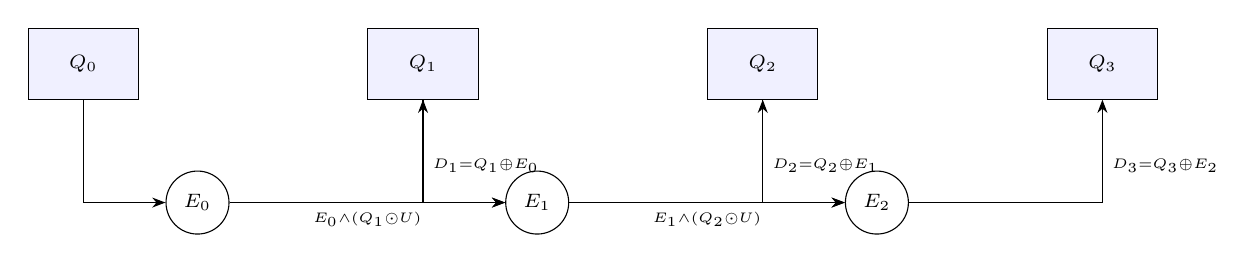
\begin{tikzpicture}[
  reg/.style={draw, minimum width=1.4cm, minimum height=0.9cm, align=center, font=\scriptsize, fill=blue!6},
  g/.style={draw, circle, minimum size=0.8cm, align=center, font=\scriptsize},
  lbl/.style={font=\tiny, align=center},
  >=Stealth, node distance=0.9cm and 2.9cm
]
  \node[reg] (r0) {$Q_0$};
  \node[reg, right=of r0] (r1) {$Q_1$};
  \node[reg, right=of r1] (r2) {$Q_2$};
  \node[reg, right=of r2] (r3) {$Q_3$};

  \node[g, below=of r0, xshift=1.45cm] (e0) {$E_0$};
  \node[g, below=of r1, xshift=1.45cm] (e1) {$E_1$};
  \node[g, below=of r2, xshift=1.45cm] (e2) {$E_2$};

  \draw[->] (r0.south) |- (e0.west);
  \draw[->] (e0) -| node[lbl,pos=0.6,above right]{$D_1{=}Q_1{\oplus}E_0$} (r1.south);
  \draw[->] (r1.south) |- (e1.west);
  \draw[->] (e0) -- (e1) node[lbl,midway,below]{$E_0{\land}(Q_1{\odot}U)$};
  \draw[->] (e1) -| node[lbl,pos=0.6,above right]{$D_2{=}Q_2{\oplus}E_1$} (r2.south);
  \draw[->] (r2.south) |- (e2.west);
  \draw[->] (e1) -- (e2) node[lbl,midway,below]{$E_1{\land}(Q_2{\odot}U)$};
  \draw[->] (e2) -| node[lbl,pos=0.6,above right]{$D_3{=}Q_3{\oplus}E_2$} (r3.south);
\end{tikzpicture}
\end{latin}
\end{center}

\paragraph*{خروجی $\mathrm{Close}$.}
\[
\mathrm{Close} = Q_0 \land Q_1 \land Q_2 \land Q_3 \quad (\text{اتاق پر، شمارش}=15)
\]
ترکیبی محض است و وضعیت لحظه‌ای شمارنده را نشان می‌دهد.

\paragraph*{قفل $\mathrm{Open}$.}
یک \lr{Register} جدا با $\mathrm{clk}=\mathrm{Clk}$، $\mathrm{en}=1$، $\mathrm{rst}=\mathrm{NCLR}$ و ورودی بعدی $\mathrm{Dopen}$:
\[
\begin{aligned}
\mathrm{LT15} &= \lnot\,\mathrm{Close} &&\text{(هنوز جا هست)}\\
\mathrm{EntValid} &= \mathrm{LT15} \land \mathrm{Ent} \land T &&\text{(درخواست معتبر)}\\
\mathrm{orr} &= \mathrm{EntValid} \lor \mathrm{Open} &&\text{(ست تازه، یا از قبل باز)}\\
\mathrm{Dopen} &= \mathrm{orr} \land \lnot\,IN &&\text{(با پالس $\mathrm{IN}$ در را ببند)}
\end{aligned}
\]
با درخواست معتبر $\mathrm{Open}$ ست می‌شود و تا آمدن $\mathrm{IN}$ از راه فیدبک روشن می‌ماند؛ همان $\mathrm{IN}$ شمارنده را هم بالا می‌برد.

\subsubsection*{مدار پیاده‌سازی‌شده}

\begin{center}
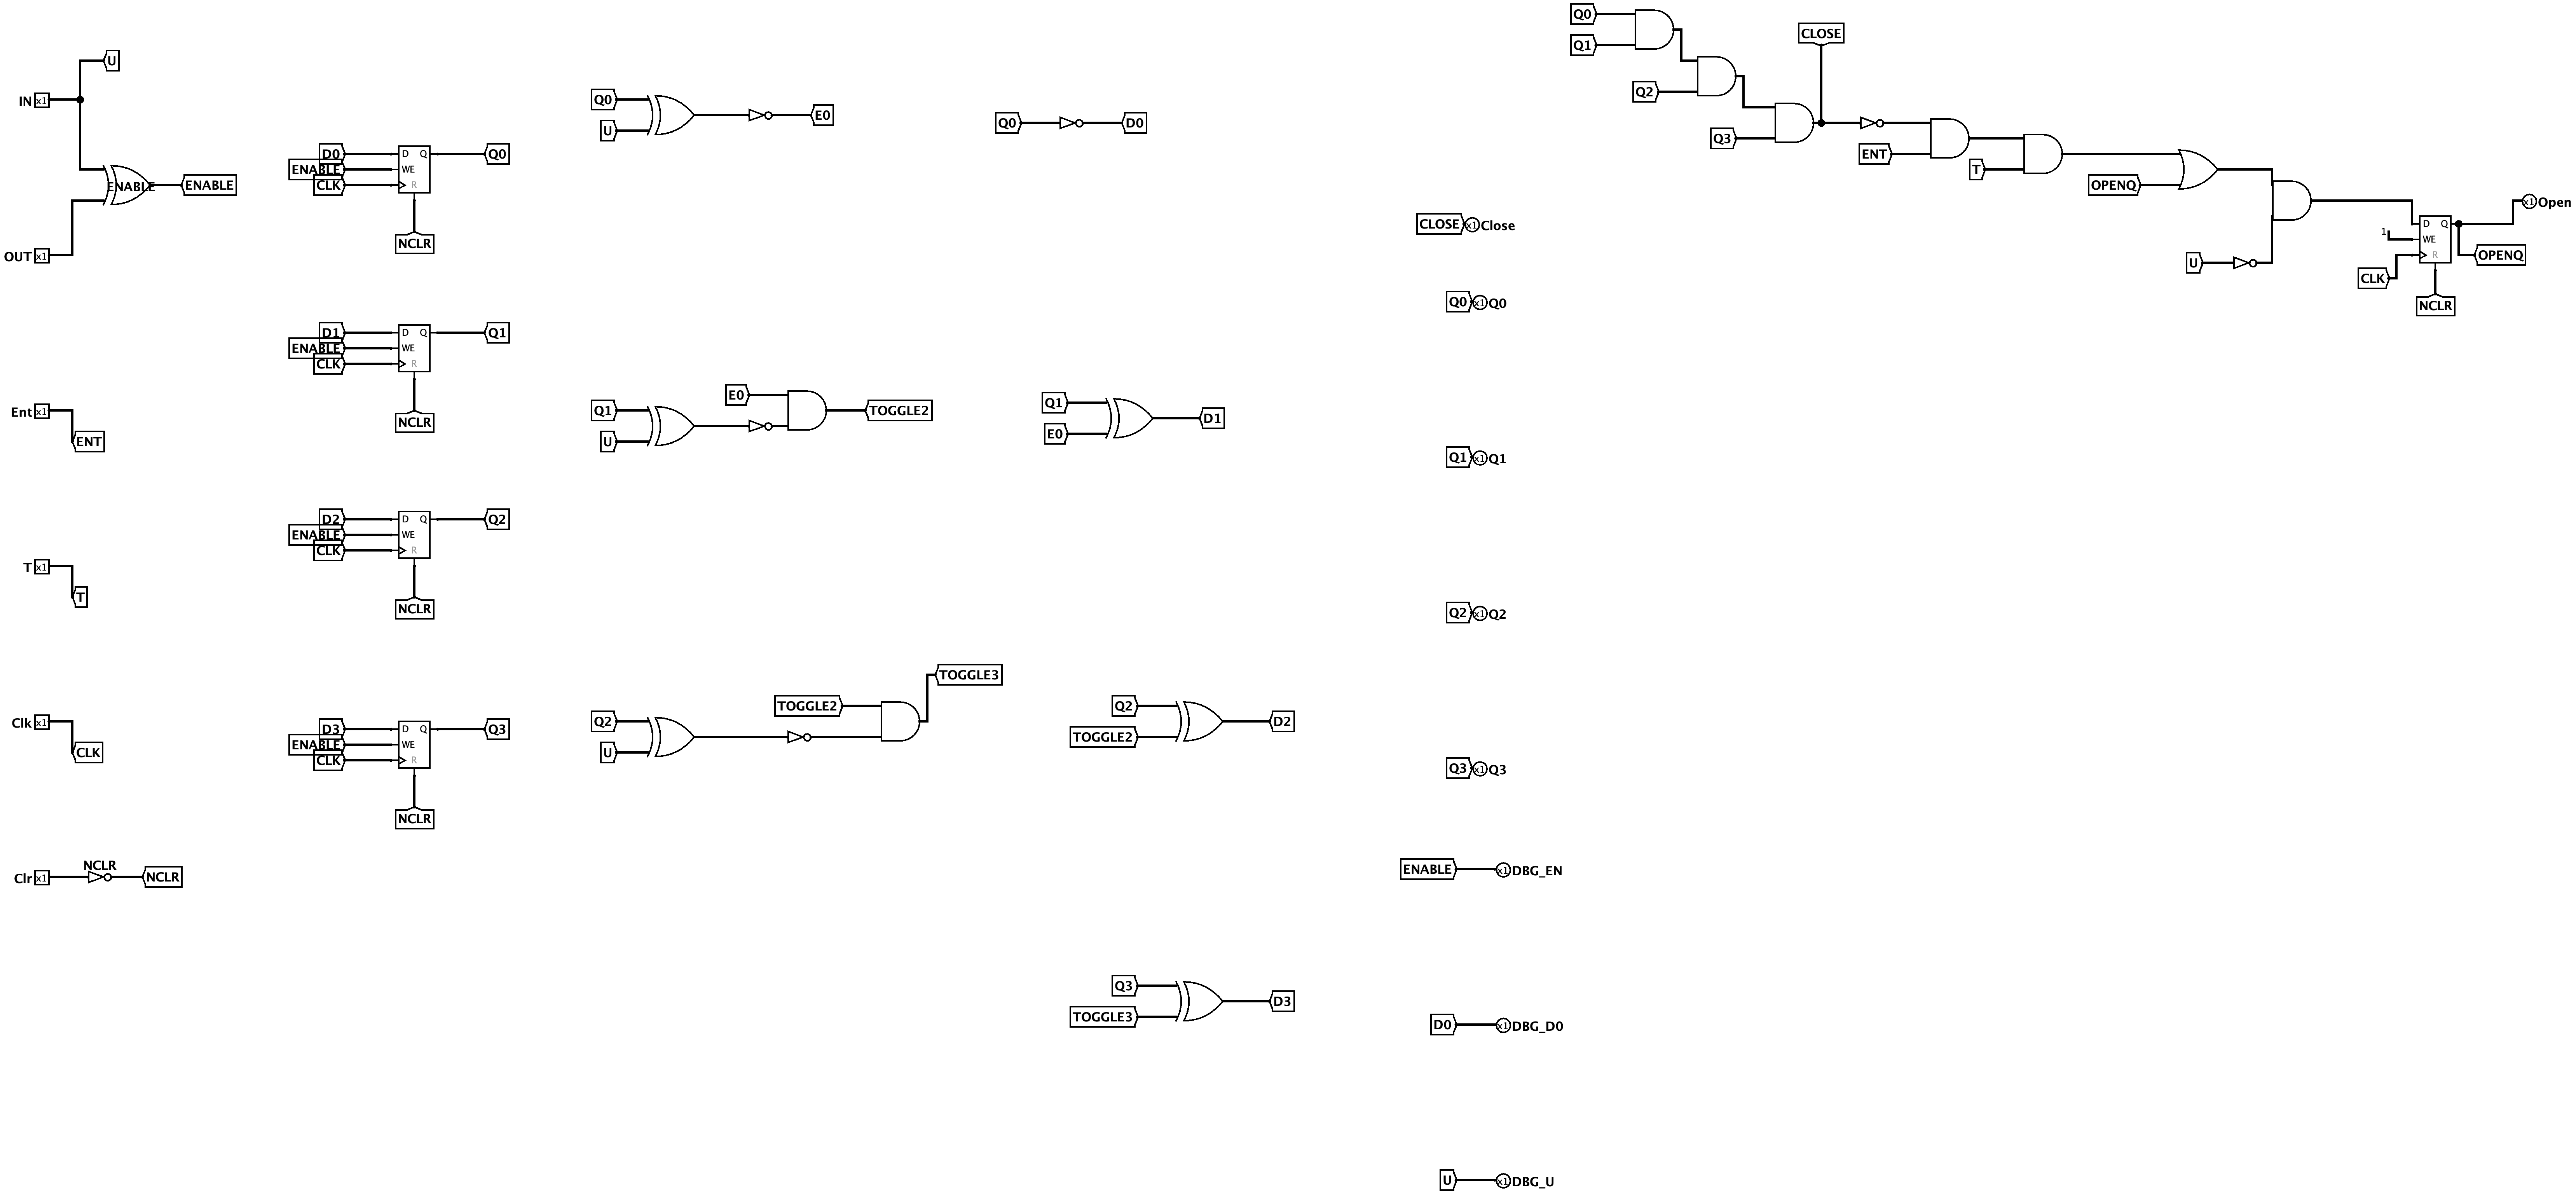
\includegraphics[width=\textwidth]{figs/pic.png}
\end{center}

\subsubsection*{نتایج تست}

مدل مرجع رفتار مدار به‌طور مستقل از خود مدار پیاده‌سازی شده و روی ۸ سناریوی هدفمند بردار تست تولید می‌کند؛ همه‌ی بردارها با اجرای واقعی \lr{Logisim} در حالت \lr{headless} (\lr{--test-vector}) روی \lr{waiting\_room.circ} تأیید شده‌اند:

\begin{center}
\begin{tabular}{@{}p{4.6cm}p{7.2cm}r@{}}
\toprule
{سناریو} & {چه چیزی را بررسی می‌کند} & {ردیف} \\
\midrule
reset-and-basic          & ریست اولیه، سکون بدون رویداد            & 7 \\
up-counting-full         & شمارش کامل ۰ تا ۱۵ با \lr{Ent}, سپس رد شدن ورودی ۱۶ام  & 63 \\
out-of-hours-blocked    & \lr{Ent} در \lr{T=0} باید همیشه رد شود        & 7 \\
exit-and-reentry         & پر شدن اتاق، خروج یک نفر، ورود دوباره     & 69 \\
simultaneous-in-out      & ورود و خروج هم‌زمان $\Rightarrow$ شمارش ثابت می‌ماند & 9 \\
open-holds-until-in     & \lr{Open} تا رسیدن پالس \lr{IN} قفل می‌ماند     & 11 \\
down-counting             & شمارش پایین‌رونده‌ی کامل تا صفر            & 21 \\
reset-mid-operation      & ریست ناهم‌گام وسط عملیات                  & 14 \\
\midrule
{جمع (\lr{tests\_waiting\_room.vec})} & & {201} \\
\bottomrule
\end{tabular}
\end{center}

خروجی واقعی اجرای \lr{run\_tests.sh}:

\begin{latin}
\lstinputlisting[basicstyle=\ttfamily\scriptsize]{figs/test_run_output.txt}
\end{latin}


\end{document}
